\documentclass[times, utf8, zavrsni, numeric]{fer}
\usepackage{booktabs}
\usepackage{nameref}
\usepackage{graphicx}
\usepackage{float}
\usepackage{natbib}
\usepackage[final]{pdfpages}

\usepackage{listings}
\usepackage{hyperref}
\lstset{frame=tb}
\graphicspath{ {c:/Users/matteom/Desktop/brzistart/slike/} }
\renewcommand{\baselinestretch}{1.5}

\begin{document}
\nocite{ungar2002uvod}
\nocite{m1}
\nocite{m2}
\nocite{WIDM:WIDM1075}
\nocite{baker2010data}

% TODO: Navedite broj rada.
\thesisnumber{5053}

% TODO: Navedite naslov rada.
\title{Primjena klasifikacijske analize u edukacijskoj domeni}

% TODO: Navedite vaše ime i prezime.
\author{Matteo Miloš}

\maketitle

% Ispis stranice s napomenom o umetanju izvornika rada. Uklonite naredbu \izvornik ako želite izbaciti tu stranicu.
\includepdf[pages=-]{slika2.pdf}

% Dodavanje zahvale ili prazne stranice. Ako ne želite dodati zahvalu, naredbu ostavite radi prazne stranice.
\zahvala{}
\hypersetup{
    colorlinks,
    citecolor=black,
    filecolor=black,
    linkcolor=black,
    urlcolor=black
}
\tableofcontents

\chapter*{Uvod}
\addcontentsline{toc}{chapter}{Uvod}

Zbog sve veće količine podataka općenito, a osobito u edukacijskoj domeni, prislijeni smo poduzeti neke mjere kako bismo izbjegli utapanje u podacima (engl. Drowning in Data). To možemo postići na način da se usmjerimo na obradu i analizu prikupljenih podataka, a ne samo na prikupljanje. Dubinska analiza podataka u edukacijskoj domeni (engl. educational data mining, EDM), iako ima neke sličnosti sa standardnom dubinskom analizom (engl. data mining, DM), zbog svoje specifičnosti često zahtijeva drukčiji pristup u analizi podataka. Kroz ovaj rad ćemo prikazati te specifičnosti i objasniti primjenu klasifikacijskih metoda nad podacima dohvaćenim iz edukacijske domene. Kao pozadinu EDM-a možemo istaknuti dvije podcjeline računarske znanosti, a to su dubinska analiza podataka (DM) i strojno učenje. Upravo njih ćemo opisati u prvim poglavljima, gdje ćemo se kod opisivanja DM-a usredotočiti na opis CRISP-DM modela dubinske analize podataka, a kod strojnog učenja glavni predmet promatranja će biti nadzirano i nenadzirano učenje, s malo većim naglaskom na nadzirano učenje. U poglavlju nakon toga, objasnit ćemo povijest razvoja EDM-a, te navesti i objasniti neke od najčešćih pristupa procesu EDM-a. Na kraju ćemo korištenjem studijskog primjera pokušati demonstrirati sve čime smo se do tada bavili na teorijskoj razini. Prije početka izvođenja primjera morat ćemo pripremiti podatkovni skup korištenjem metoda koje smo prethodno opisali kod opisa CRISP-DM modela, a nakon što smo skup pripremili, korištenjem dva algoritma klasifikacijske analize, logističke regresije i algoritma k-najbližih susjeda (KNN), prikazat ćemo ovisnost uspjeha studenata o pojedinim atributima koji ih karakteriziraju.

\chapter{Dubinska analiza podataka}
\section{Općenito i nastanak}
U današnjem svijetu, dubinska analiza podataka (engl. data mining) se nameće kao bitan termin prilikom razgovora o podatkovnoj analizi. Dubinska analiza podataka u svojoj definiciji obuhvaća obradu i sortiranje velikih podatkovnih skupova, kako bi se identificirali neki uzorci i uspostavile veze među podacima. Uz upravo spomenuto, glavni cilj dubinske analize podataka je izvlačenje korisnih informacija iz podatkovnog skupa i njihovo pretvaranje u razumljivu strukturu kako bi one bile korisne u nekim daljnjim analizama. Iz prethodno navedenog, gdje vidimo da je glavni cilj izvlačenje, odnosno rudarenje informacija, mogli bismo dati i precizniji naziv za rudarenje podataka koji bi glasio: "rudarenje znanja iz podataka". Dubinska analiza podataka je proces koji obuhvaća mnoge grane znanosti, a kao najvažnije možemo istaknuti: strojno učenje, umjetnu inteligenciju i statistiku\cite{SAM:SAM10000}.

Kako bismo objasnili potrebu za dubinskom analizom podataka, moramo iznijeti pozadinu cijele priče. U današnjem svijetu, prema procjeni IBM-a, pretpostavlja se da se svaki dan kreira oko 2.5 kvintilijuna $(2.5*10^{18})$ bajtova podataka\cite{ibm}. Nadalje, od svih podataka u svijetu, otprilike 90\% je nastalo u zadnje 2 godine. Ti podaci dolaze iz raznih izvora kao što su: društvene mreže na internetu, fotografije i videozapisi, signali koje odašiljaju GPS uređaji i sl.. Nastave li podaci rasti ovim tempom,  pretpostavka je da će u svijetu do 2020. godine postojati oko 40 zetabajtova $(40*10^{21})$ podataka. Iz te silne količine podataka nastao je i termin big data koji ovom prilikom nećemo preciznije objašnjavati. Potreba za dubinskom analizom je došla u onom trenutku kada su ljudi shvatili da, bez obzira na to koliko mnogo podataka posjedovali oni sami po sebi ništa ne znače. Kako bi izvukli neku vrijednost iz njih, odnosno informaciju, potrebno je pronaći razne načine za obradu tih podataka te se tako rodila dubinska analiza podataka.	
\section{Proces dubinske analize podataka}
U znanstvenoj literaturi se osim termina dubinska analiza podataka, često zna i pojaviti termin "otkrivanje znanja iz baza podataka" (engl. Knowledge Discovery in Databases-KDD). KDD je okvirno podijeljen na 5 faza koje su:
\begin{enumerate}
\item Selekcija
\item Pretprocesuiranje
\item Transformacija
\item Dubinska analiza
\item Interpretacija i evaluacija
\end{enumerate}
Ipak, jedan od najkorištenijih modela koji opisuju dubinsku analizu podataka je CRISP-DM(engl. CRoss Industry Standard process for Dana Mining). Taj model je nastao na osnovu iskustava raznih ljudi u praktičnoj primjeni iz vodećih svjetskih tvrtki. Slika 1 pobliže opisuje ovaj model i prikazuje najbitnije faze standardnog procesa i njihov redoslijed. Međutim, kod redoslijeda faza nije strogo određen te često može doći do situacije da se iz sljedeće faze moramo vratiti jedan ili više koraka unatrag. Taj odnos međuovisnosti faza je prikazan strelicama na Slici~\ref{fig:crisp-dm}.

\begin{figure}[htb]
\centering
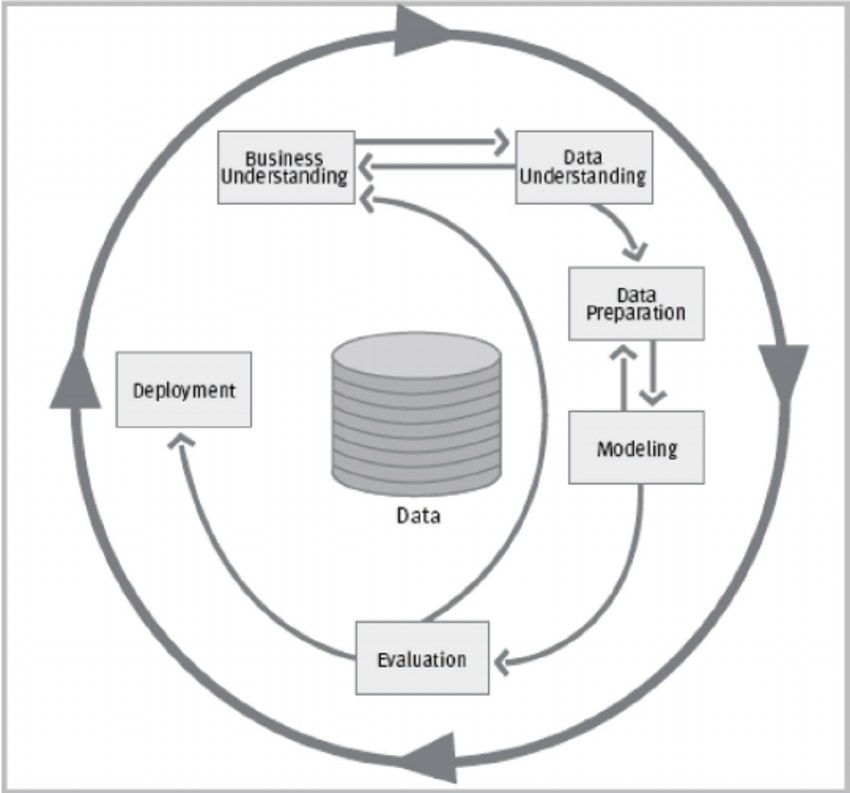
\includegraphics[width=6cm, height=5cm]{CRISP.jpg}
\caption{Faze modela CRISP-DM\cite{m3}}
\label{fig:crisp-dm}
\end{figure}
\newpage
\section{Opis CRISP-DM modela dubinske analize podataka}\label{chap:begin}
Kao što je prikazano na Slici~\ref{fig:crisp-dm}, model CRISP-DM razbija proces analize na 6 glavnih faza. Tih 6 faza ćemo se sada pobliže objasniti
\begin{enumerate}
\item \textbf{Razumijevanje problema}
\end{enumerate}
U fazi razumijevanja problema, problemu pristupamo na način da ga pokušavamo sagledati iz poslovne perspektive, ali i iz perspektive primjene tehnika dubinske analize podataka. Gledanjem kroz ta dva aspekta i njihovim ujedinjavanjem dolazimo do definicije problema i određivanja konačnih ciljeva. Nakon toga dolazimo i do zadnjeg dijela prve faze, a to je izrada okvirnog plana. Plan osim aktivnosti koje će se provoditi sadrži i procjenu cijene i trajanja postupka. Iako se ovaj prvi korak čini manje bitan, njegovo zanemarivanje može dovesti do toga da se sav trud uloži u traženje odgovora na kriva pitanja.\cite{crisp1}\cite{crisp2}
\begin{enumerate}[resume]
\item \textbf{Razumijevanje podataka}
\end{enumerate}
U ovoj fazi se usmjeravamo na ono zbog čega i radimo analizu, a to su podaci. Samu fazu razumijevanja podataka također možemo podijeliti na dva dijela. Prvi dio obuhvaća utvrđivanje opsega podataka i njihovo inicijalno prikupljanje. Faza prikupljanja se nastavlja na aktivnosti u kojima se pokušavamo upoznati s podatkovnim skupom jednostavnijim statističkim metodama kao što su primjerice standardna devijacija ili aritmetička sredina. Nakon toga, dolazimo do dijela koji je priprema za treću fazu CRISP-DM modela, a to je verifikacija kvalitete podataka. Ona obuhvaća kompleksnije upoznavanje s podacima na način da provjeravamo konzistentnost podataka te tražimo neke šumove, odnosno pogreške u podacima koje ćemo pokušati otkloniti u sljedećoj fazi..\cite{crisp1}\cite{crisp2}
\begin{enumerate}[resume]
\item \textbf{Priprema podataka}
\end{enumerate}
Treća faza je vremenski najopsežnija faza dubinske analize podataka pa ćemo ju i pokušati najpreciznije opisati. Nakon što smo u prošloj fazi prikupili i upoznali se s podacima, na početku ove faze dolazi korak odabira podataka. Tu odabiremo neki podskup iz skupa svih podataka koji će najbolje poslužiti za daljnju analizu. Pri tome u obzir uzimamo koliko su nam bitni neki atributi u podatkovnom skupu (nebitne izbacujemo) te potpunost opisanih stupaca i redaka u skupu kojeg obrađujemo. Zatim nastavljamo s pročišćavanjem podataka koje se nadopunjuje na prethodni korak. Proces pročišćavanja najbolje možemo opisati Tablicom~\ref{fig:pripremapod}:\\

\begin{table}[htb]
\caption{Pročišćavanja podataka}
\begin{tabular}{| l | p{8cm} |}
    \hline
    \textbf{PROBLEM S PODACIMA} & \textbf{MOGUĆE RJEŠENJE} \\ \hline
    Podaci nedostaju & Izbacivanje nepotpunih redaka ili popunjavanje praznina s pretpostavljenim vrijednostima \\ \hline
    Greške u podacima & Koristeći logiku otkrivamo pogreške te ih ispravljamo ukoliko je to moguće ili izbacujemo retke s greškama\\ \hline
    Neprikladne vrijednosti atributa & Normaliziranje (npr. svođenje vrijednosti numeričkih atributa na interval [0,1]) ili zaglađivanje podataka (diskretizacija numeričkih atributa) \\
    \hline
\end{tabular}
\label{fig:pripremapod}
\end{table}
Nakon što smo na navedeni način pročistili podatke, pokušat ćemo iz odabranih i pročišćenih podataka konstruirati nove podatke. To možemo učiniti na dva načina, deriviranjem postojećih atributa, što podrazumijeva kreiranje novih atributa iz postojećih (npr. površina = širina * visina), ili generiranjem novih redaka, iako pri potonjoj metodi moramo biti pažljivi te promisliti je li nam ona uopće potrebna. Kao zadnji korak prije faze modeliranja možemo navesti formatiranje, odnosno oblikovanje podataka. Taj proces je više tehničke prirode i kao primjer možemo uzeti sortiranje podataka prije njihove obrade.\cite{crisp1}\cite{crisp3}
\begin{enumerate}[resume]
\item \textbf{Modeliranje podataka}
\end{enumerate}
Modeliranje podataka je faza koja je vjerojatno najdraža većini podatkovnih analitičara. To je točka u kojoj sav dosadašnji trud počinje dolaziti na vidjelo. Za početak, moramo odabrati tehnike modeliranja, a pri tom odabiru ćemo uzeti sljedeće stvari:
\begin{itemize}
\item koji tipovi podataka su dostupni za analizu
\item koji su konačni ciljevi dubinske analize podataka
\item odnos karakteristika promatranog problema i različitih tehnika modeliranja
\end{itemize}
Nakon odabranih tehnika, prije same izgradnje modela, prvo moramo konstruirati mehanizam kojim ćemo testirati kvalitetu i valjanost kasnije napravljenog modela. Primjerice, dobrota (engl. goodness) modela tipično se ocjenjuje stopom pogreške određenog modela. Konačno, nakon izrađenih testova, dolazimo do dijela koji je najzanimljiviji i koji mnogi neupućeni u tematiku shvaćaju kao jedini dio dubinske analize podataka, a to je izgradnja modela. U tom procesu ne dolazi do izrade jednog modela, već se, u pravilu, generira veći broj različitih modela. Ti modeli očekivano variraju po svojoj kvaliteti i obliku, pa se raznim iterativnim postupcima pokušavaju izdvojiti oni najkvalitetniji i najpogodniji za željeni cilj. Tim postupkom završava faza modeliranja podataka te nakon toga dolazimo do dvije mogućnosti, ili prelazimo na sljedeću fazu evaluacije, ili se po potrebi, kao što je prikazano na Slici~\ref{fig:crisp-dm}, vraćamo u fazu pripremanja podataka.\cite{crisp2}\cite{crisp3}
\begin{enumerate}[resume]
\item \textbf{Evaluacija modela}
\end{enumerate}
U trenutku dolaska u fazu evaluacije modela, može se reći da je većina analize obavljena. Kao što sam naziv kaže, u ovoj fazi evaluiramo analizirane podatke i ocjenjujemo jesmo li izrađenim modelom postigli ono što smo definirali još u prvoj fazi, a to su ciljevi promatrani s poslovne strane. Pri tome se vodimo sljedećim pitanjima:
\begin{itemize}
\item jesu li rezultati dobiveni u formi koja se može lako prikazati
\item ima li nekih jedinstvenih otkrića koje bi trebalo posebno istaknuti
\item možemo li rangirati izrađene modele po njihovoj poslovnoj svrsi
\item koliko dobro izrađeni modeli odgovaraju početno zadanom poslovnom cilju
\item jesu li navedena ispitivanja pobudila neka nova, neodgovorena pitanja
\end{itemize}
Ukoliko naša ocjena modela, vođena prethodno navedenim pitanjima, nije zadovoljavajuća, postoji mogućnost povratka skroz na početak, odnosno u fazu razumijevanja problema kao što je prikazano na dijagramu na Slici~\ref{fig:crisp-dm}.\cite{crisp2}
\begin{enumerate}[resume]
\item \textbf{Primjena rezultata}
\end{enumerate}
U ovoj fazi dolazi do konačne isplativosti cijelog procesa analize. Ipak, prije same primjene, moramo kreirati i njezin plan. Ta procedura podrazumijeva izradu strategije primjene, potrebnih koraka i instrukcija za provođenje tih koraka. Nakon toga počinjemo s primjenom rezultata te paralelno određujemo na koji ćemo način pratiti i održavati performanse našeg modela, te po potrebi, ukoliko dođe do opadanja uspjeha modela, provesti novu analizu. Kao logičan završetak cijelog proces, možemo navesti završni izvještaj u kojem radimo kratki sažetak kako rezultata projekta, tako i svi pretpostavki i akcija koje su poduzete u dolasku do rezultata.


\chapter{Strojno učenje}
\section{Općenito, nastanak i razvoj}
Jedna od najzanimljivijih, ali vjerojatno i najrazvijenijih područja računarske znanosti je strojno učenje (engl. machine learning). Iako mnogi, kada čuju taj pojam, često pomisle na znanstveno-fantastične filmove u kojima razvoj strojnog učenja za sobom neizbježno vodi ratu između strojeva i njihovih stvaratelja, u stvarnosti on predstavlja nešto sasvim drugo. Mogućnosti primjene strojnog učenja sežu od raspoznavanja uzoraka i dubinske analize podataka, koji su najviše obrađeni u ovom radu, do robotike, računalnog vida, bioinformatike i računalne lingvistike. Uz to, kao tri osnovna pristupa strojnom učenju možemo navesti nadzirano i nenadzirano učenje te podržano učenje, koji će detaljnije biti obrađeni kasnije. Prije toga, pokušat ćemo objasniti razvoj i razloge razvoja strojnog učenja. Strojno učenje nastalo je u okruženju u kojem su dostupni podaci, statističke metode, ali i moć računala u simultanom i eksponencijalnom porastu. Povećanje količine podataka je nužno za sobom povuklo razvoj računala, što je zatim dovelo do napretka kod statističkih metoda za analiziranje velikih podatkovnih skupova, koje smo spomenuli na početku ove rečenice. Dakle, možemo zaključiti da se kreirao krug koji je ciklički stvarao napredak te 3 cjeline. To si možemo lakše dočarati koristeći ilustraciju na Slici~\ref{fig:strojnokrug}.

\begin{figure}[H]
\centering
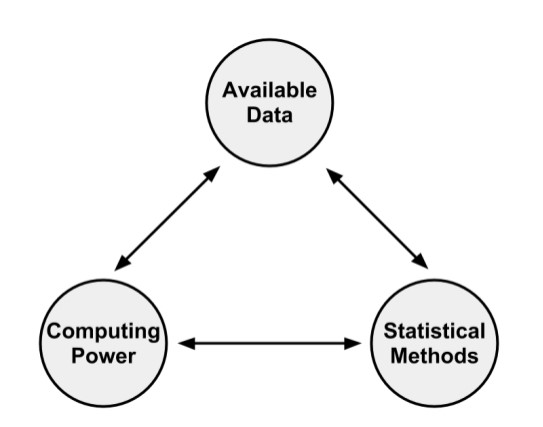
\includegraphics[width=6cm]{strojnoKrug.jpg}
\caption{Proces koji je izazvao razvoj strojnog učenja\cite{ungar2002uvod}}
\label{fig:strojnokrug}
\end{figure}

Svu tu količinu podataka bilo je potrebno na neki način "obuzdati", te se tako razvilo strojno učenje čije je polje interesa bilo usmjereno prema računalnim algoritmima za pretvaranje podataka u inteligentne radnje. U početku, strojno učenje počelo je izrastati iz umjetne inteligencije, kada su brojni istraživači pokazali interes u kreiranju strojeva koji mogu učiti iz danih podataka. Iako je u startu, u 50-im godinama 20. stoljeća, nakon Turingova stroja koji je imao sposobnost učenja, interes za strojnim učenjem bio vrlo visok, u 70-im godinama dolazi do takozvanog perioda zime (engl. AI Winter) za umjetnu inteligenciju. Uzevši u obzir da su dana umjetna inteligencija i strojno učenje bili vrlo duboko povezani, ta zima označila je stagnaciju i za strojno učenje. Do perioda stagnacije došlo je iz razloga što znanstvenici nisu uspjeli u malom vremenskom razmaku ostvariti veliki napredak kod učenja računala, te je došlo do bojazni da su se približili vrhuncu znanja o strojnom učenju. Ipak, do uskrsnuća ove grane računarske znanosti došlo je desetak godina kasnije nakon otkrića novog algoritma neuronskih mreža, mreža širenjem unatrag (engl. backpropagation). Nakon toga, strojno učenje se sve više počelo usmjeravati prema tome da u nečemu nadmaši čovjeka, pa smo tako 1997. svjedočili prvoj pobjedi računala nad svjetskim šahovskim prvakom. Od novijih dostignuća, vrijedi spomenuti prvu pobjedu računala u igri Go iz 2016. godine, gdje je računalo koristeći tehnike strojnog učenja i pretraživanja stabla nadmašilo prvaka u toj igri.

\section{Podjela strojnog učenja}
Kao što smo već ranije spomenuli, ovisno o tome sadrži li sustav za učenje pripremljene primjere, strojno učenje dijelimo na 3 kategorije koje su: nadzirano učenje, nenadzirano učenje, podržano učenje. Od ovih kategorija, najzastupljenije je nadzirano učenje, pa ćemo sukladno tome njega i najdetaljnije obraditi.
\subsection{Nadzirano učenje}
Nadzirano učenje je potkategorija strojnog učenja koja podrazumijeva da sustav sadrži pripremljeni skup za učenje (engl. training set) koji sadrži testne primjere. Testne primjere možemo predočiti kao par ($x$,$y$), gdje $x$ predstavlja vektor spripremljenim ulaznim parametrima, a $y$ predstavlja vrijednost koju želimo dobiti nakon obrade vektora $x$. U optimalnom slučaju, algoritam učenja će zadovoljiti sve pripremljene testne primjere, ali će također biti u mogućnosti  uspješno riješiti i primjere koji mu nisu bili omogućeni u skupu za učenje. Da bi ostvario tu mogućnost, algoritam mora izbjeći učenje "napamet" pripremljenih primjera već mora pronaći neku logiku, odnosno funkciju kojom će doći do željenog rezultata i tako biti spreman na nove, dosad neviđene primjere. Okvirno, metode nadziranog učenja možemo podijeliti na 2 dijela: klasifikaciju i regresiju. U razradi, više vremena ćemo posvetiti objašnjavanju klasifikaciji jer je ovaj rad orijentiran upravo na tu metodu.\cite{super1}\cite{super2}
\let\labelitemi\labelitemii
\begin{itemize}
  \item \textbf{KLASIFIKACIJA}
\end{itemize}
Klasifikaciju definiramo kao problem određivanja kojem podskupu rezultata pripada određeno zapažanje nad nekim podacima. Pri tom određivanju, uzevši u obzir da ova metoda pripada nadziranom učenju, koristi se skup za učenje. Kao jednostavan primjer klasifikacije možemo uzeti određivanje prolaznosti studenta na kolegiju. Kao što se može i pretpostaviti, imamo dva podskupa rezultata, a to su prolaz i pad. Kao zapažanje, možemo koristiti razne parametre kao što su primjerice: dolaznost studenta na predavanja, aktivnost studenta na predavanju, dosadašnji prosjek studenta na fakultetu, studentov socijalni status i slično. Dakle, klasifikaciju također možemo definirati kao prepoznavanje određenog uzorka nad ulaznim zapažanjima. Algoritam koji implementira metodu klasifikacije nazivamo klasifikatorom. Postoje dvije vrste klasifikatora, a to su binarni klasifikator i višeklasni klasifikator. Binarni klasifikator se koristi u situacijama kada želimo ograničiti dobiveni rezultat u dvije klase, pa ga često možemo predočiti Booleovom funkcijom, gdje jedna klasa predstavlja vrijednost 1, a druga klasa vrijednost 0. Gore navedeni primjer prolaznosti studenta bi koristio binarni klasifikator. Višeklasni klasifikator, kao što mu i samo ime govori, koristi se kada želimo rezultate podijeliti u više klasa, primjerice ako radimo klasifikaciju filmova po žanrovima ili klasifikaciju prijenosnih računala po veličini. Kod klasifikacije, uvodimo i pojam model ili prostor hipoteza, koji predstavlja skup svih mogućih hipoteza $H$. Učenje se zapravo svodi na pretraživanje prostora hipoteza $H$ i pronalaženje najbolje hipoteze $\hslash$ $\varepsilon$ $H$. Dakako, najbolja hipoteza je ona koja najtočnije klasificira zadane primjere. Točnost svake hipoteze najbolje možemo ocijeniti empirijskom pogreškom. Empirijska pogreška hipoteze $\varepsilon$, mjerena na skupu $D$, jednaka je udjelu primjera iz $D$ koji nisu ispravno klasificirani:
\begin{equation}
E(\hslash|D)=\frac{1}{N}\sum_{i=1}^{N}f\{\hslash(x^{(i)})\neq y^{(i)}\} = \frac{1}{N}\sum_{i=1}^{N}|\hslash(x^{(i)}) - y^{(i)}|
\end{equation}
,gdje je $f$\{$P$\} indikatorska funkcija čija je vrijednost 1 ako je $P$ = T, a 0 inače. Primjeri koje hipoteza klasificira pozitivno, a pripadaju negativnom skupu, nazivamo lažno pozitivnim primjerima (engl. false positives). Obrnute primjere, odnosno primjere koji pripadaju negativnom skupu, a hipoteza ih klasificira pozitivno, nazivamo lažno negativnim primjerima (engl. false negatives). Kod klasifikacije, često dolazi do slučaja da za neki skup za učenje $D$, pronalazimo više hipoteza koje ispravno klasificiraju zadane primjere iz skupa za učenje. Skup takvih hipoteza nazivamo prostor inačica (engl. version space)\cite{skrip}. Skup prostor inačica moguće je podijeliti u dva skupa hipoteza, a to su: 
\begin{enumerate}
\item skup najspecifičnijih konzistentnih hipoteza
\item skup najopćenitijih konzistentnih hipoteza
\end{enumerate}
gdje "konzistentnih" znači da hipoteze pokrivaju sve pozitivne i nijedan negativni slučaj. Prvi skup definiramo tako da kažemo da on pokriva sve pozitivne slučajeve na način da zauzme što je manje prostora moguće. Ukoliko bi došlo do smanjivanja skupa za neki najminimalniji dio, skup bi postao nekonzistentan jer bi prestao pokrivati neki pozitivan slučaj. Drugi skup, skup najopćenitijih konzistentnih hipoteza, definiramo na način da on pokriva sve pozitivne slučajeve, ali i koliko god je moguće još prostora dokle god ne dolazi do negativnih slučajeva. Ukoliko bi došlo do povećanja tog skupa za neku minimalnu vrijednost, skup bi postao nekonzistentan jer bi se unutar njega našao i neki nedozvoljeni negativni slučaj. To najbolje možemo objasniti ilustracijom na Slici~\ref{fig:speciopc}, gdje oznaka SB predstavlja prvi skup, a oznaka GB drugi skup. 

\begin{figure}[H]
\centering
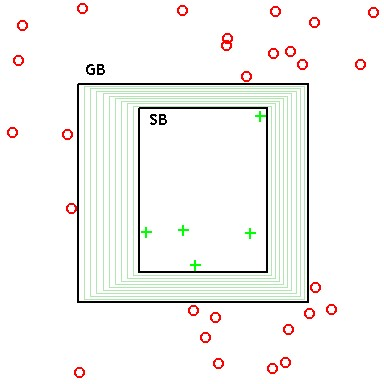
\includegraphics[width=7cm]{speciopc.jpg}
\caption{Podjela skupa prostor inačica)\cite{skrip}}
\label{fig:speciopc}
\end{figure}


Postupak klasifikacije se najčešće izvodi korištenjem klasifikacijskog stabla, ali pri tome treba paziti da izgrađeno stablo ne bude prekompleksno, ali ni prejednostavno. Dobar primjer za navedene slučajeve dat ćemo analizirajući skup za učenje na Slici~\ref{fig:skupuc}

\begin{figure}[H]
\centering
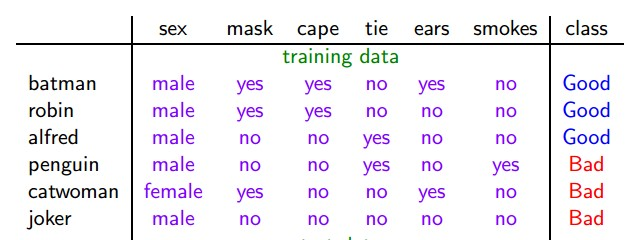
\includegraphics[width=7cm]{skupuc.jpg}
\caption{Primjer klasifikacije, skup za učenje\cite{pic}}
\label{fig:skupuc}
\end{figure}

Na Slici~\ref{fig:skupuc} je prikazan kratak opis izgleda raznih (anti)junaka iz američkog stripovskog serijala Batman. Cilj je izgraditi klasifikator koji bi na temelju zadanih atributa mogao odrediti ima li neki lik dobru ili lošu ulogu. Kao primjer loših klasifikatora, mogli bi navesti sljedeća 2 primjera. 

\begin{figure}[H]
\centering
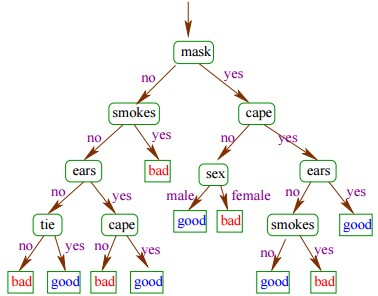
\includegraphics[width=7cm]{overfit.jpg}
\caption{Loš primjer klasifikatora zbog prenaučenosti\cite{pic}}
\label{fig:overfit}
\end{figure}

\begin{figure}[H]
\centering
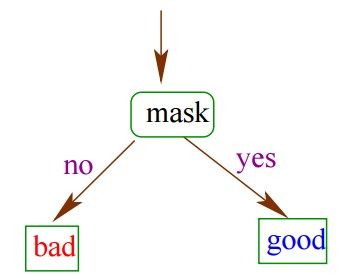
\includegraphics[width=7cm]{underfit.jpg}
\caption{Loš primjer klasifikatora zbog podnaučenosti\cite{pic}}
\label{fig:underfit}
\end{figure}

Već intuitivno, možemo procijeniti da klasifikator na Slici~\ref{fig:overfit} nije odgovarajući jer je prekompleksan, iako savršeno klasificira zadani skup. Tu također dolazi do problema prenaučenosti (engl.overfitting), odnosno problema kod kojeg naš klasifikator radi preopćenito stablo prema skupu za učenje, i onda lako dolazi do pogreške kod bilo kakvog drugog primjera. Drugi pak klasifikator, na Slici~\ref{fig:underfit}, iako je vrlo jednostavan, nije dovoljno precizan upravo zbog svoje jednostavnosti i kod njega dolazi do problema podnaučenosti (engl.overfitting). Kao dovoljno precizan, ali i dovoljno jednostavan klasifikator za gore navedeni problem, možemo navesti primjer na Slici~\ref{fig:dobarklas}
\begin{figure}[H]
\centering
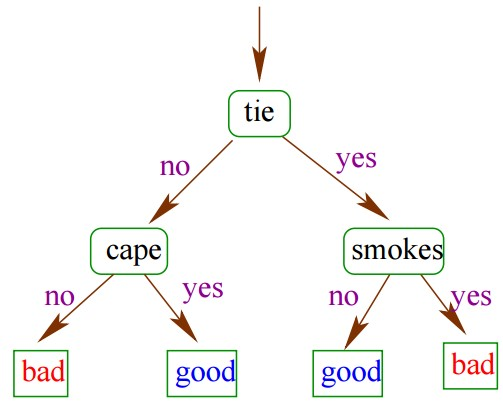
\includegraphics[width=10cm]{dobarklas.jpg}
\caption{Primjer dobrog klasifikatora\cite{pic}}
\label{fig:dobarklas}
\end{figure}
Također, možemo primijetiti i da bi se ovaj klasifikator izvrsno ponašao i pri klasifikaciji dosad neviđenih likova iz testnog skupa sa Slike~\ref{fig:testskup} , gdje bi ispravno lik "batgirl" klasificirao kao dobar, a lik "riddler" kao loš.

\begin{figure}[H]
\centering
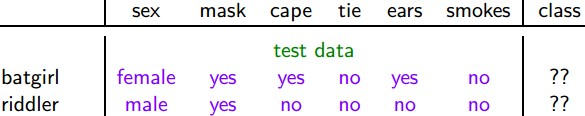
\includegraphics[width=10cm]{testskup.jpg}
\caption{Skup za testiranje klasifikatora\cite{pic}}
\label{fig:testskup}
\end{figure}

\let\labelitemi\labelitemii
\begin{itemize}
  \item \textbf{REGRESIJA}
\end{itemize}

Regresija, za razliku od klasifikacije kod koje je ciljna vrijednost iz diskretnog skupa, pokušava odrediti rezultat $y$ čija je vrijednost kontinuirana i vrijedi $y$ $\epsilon$ $R$. Kao i klasifikacija, i regresija u svom procesu koristi skup za učenje. Za jednostavan primjer regresije, također ćemo uzeti u obzir uspješnost nekog studenta na pojedinom kolegiju. Međutim, ovaj put nećemo prognozirati vrijednosti iz diskretnog skupa (prolaz/pad), već ćemo prognozirati numeričke kontinuirane vrijednosti (broj bodova). Dakle, u obzir bismo uzeli, kao i kod klasifikacije, neke parametre vezano za studenta, njegovu dolaznost i aktivnost na predavanjima, broj napisanih zadaća, živi li s roditeljima ili samostalno i slično. Na temelju tih parametara, naš algoritam bi morao ispravno procjenjivati koliki će biti konačni uspjeh, odnosno koliko će bodova student ostvariti na nekom kolegiju. Kao jednostavan primjer možemo navesti stablo na Slici~\ref{fig:regprim} (svi podaci sa slike su potpuno izmišljeni).

\begin{figure}[H]
\centering
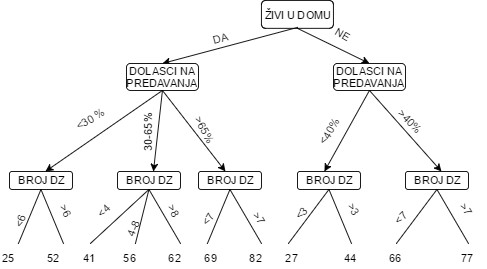
\includegraphics[width=10cm]{regprim.jpg}
\caption{Primjer regresijskog stabla za uspjeh studenata}
\label{fig:regprim}
\end{figure}
Govoreći o regresiji, ono što ne smijemo zaboraviti je istaknuti nekoliko najkorištenijih postupaka regresije. U slučaju da neka hipoteza $\hslash$, iz prostora hipoteza $H$, linearno ovisi o ulaznim vrijednostima $x$, tada govorimo o linearnoj regresiji. Zbog jednostavnosti, pretpostavit ćemo da je prostor ulaznih vrijednosti $X$ jednodimenzijski, odnosno da se radi o jednostavnoj linearnoj regresiji. Tada je hipoteza $\hslash$ definirana jednadžbom pravca 
\begin{equation}
\hslash(x) = \omega_1 x + \omega_0
\end{equation}
gdje $\omega_1$ predstavlja regresijski koeficijent, a $\omega_0$w0 konstantni član, odnosno očekivanu vrijednost zavisne varijable kad je nezavisna varijabla jednaka nuli\cite{skrip}.
U tom slučaju, empirijska pogreška je:
\begin{equation}
E(\hslash|D)=\frac{1}{2}\sum_{i=1}^{N}(y^{(i)}-(\omega_1 x^{(i)} + \omega_0))^2
\end{equation}
Očekivano, naš cilj je pronaći hipotezu $\hslash$ koja minimizira emipirijsku pogrešku. Budući da je empirijska pogreška dana kao zbroj kvadrata pogrešaka koje nastaju na pojedinačnim primjerima, riječ je o postupku najmanjih kvadrata (engl. least square method). Rješavanjem diferencijalnih jednadžbi s obzirom na parametre $\omega_0$ i $\omega_1$, dolazimo do rješenja koja su
\begin{equation}
\omega_0=\bar{y}-\omega_1 \bar{x}
\end{equation}

\begin{equation}
\omega_1=\frac{\sum_{i=1}^{N} x^{(i)} y^{(i)} - N \bar{x}\bar{y}}{\sum_{i=1}^{N} (x^{(i)})^2 - N \bar{x}^2}
\end{equation}
U slučajevima kada je linearan model prejednostavan dolazi do prevelike empirijske pogreške. Tada možemo odabrati mogućnost polinomijalne regresije, a kao primjer ćemo uzeti polinom drugog reda:
\begin{equation}
\hslash(x)=\omega_2 x^2 + \omega_1 x + \omega_0
\end{equation}
Usporedbu analize linearnom i polinomijalnom regresijom možemo vidjeti na Slici~\ref{fig:usporedba}

\begin{figure}[H]
\centering
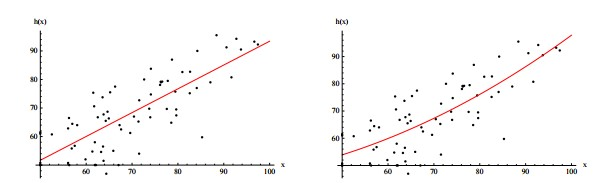
\includegraphics[width=10cm]{usporedba.jpg}
\caption{Usporedba linearne i polinomijalne regresije\cite{skrip}}
\label{fig:usporedba}
\end{figure}

\subsection{Nenadzirano učenje}
Dok kod nadziranog učenja na raspolaganju imamo skup za učenje kod kojeg za svaki primjer $x$ imamo označenu ciljnu vrijednost $y$, kod nenadziranog učenja te ciljne označene vrijednosti nema. To se najčešće događa iz razloga što je označivanje ciljne vrijednosti vremenski skup postupak. Nenadzirano učenje (engl. unsupervised learning) se najčešće oslanja tri tipična zadatka, a to su: grupiranje (engl. clustering), otkrivanje novih vrijednosti ili vrijednosti koje odskaču (engl. novelty/anomaly detection) i smanjenje dimenzionalnosti (engl. dimensionality reduction). U nastavku ćemo se kratko osvrnuti na svaki od navedenih zadataka.

\begin{itemize}
\item \textbf{GRUPIRANJE}
\end{itemize}
Grupiranje je proces koji se fokusira na razdjeljivanje zadanih primjera u grupe primjera, tako da uzimamo u obzir sličnost primjera po nekom svojstvu. Samo grupiranje se ne izvodi nekim određenim algoritmom, već se svodi na primjenjivanje više različitih algoritama pa ga svrstavamo u probleme višekriterijske optimizacije. Algoritmi koji će se koristiti kod grupiranja se određuju ovisno o zadanom podatkovnom skupu i o željenoj namjeri s dobivenim rezultatima. Od mnogih vrsta grupiranja izdvojit ćemo dva načina, a to su: grupiranje k-srednjim vrijednostima (engl. k-means clustering) i hijerarhijsko grupiranje (engl. hierarchical clustering). Grupiranje k-srednjim vrijednostima se najčešće oslanja na Lloydov algoritam. Algoritam se najbolje može opisati na ovaj način\cite{lloyd}:

\begin{enumerate}
\item	Odaberi proizvoljno (slučajno) k točaka (to mogu biti i konkretni primjeri iz skupa podataka!) kao početne točke centroide svih k grupa
\item Pridijeli svaki primjer centroidu kojem je primjer najbliži, formirajući na taj način k ekskluzivnih grupa primjera
\item Izračunaj nove centroide grupa i to na taj način da usrednjiš, po pojedinim atributima, vrijednosti svih primjera koji pripadaju određenoj grupi, 
odnosno (centroidu).
\item Provjeri da li su centroidi grupa promijenili svoje "koordinate" iznad prethodno definiranih minimalnih vrijednosti. Ako jesu, kreni iznova od točke 2. Ako ne, određivanje grupa je završeno, (svi primjeri pridijeljeni su odgovarajućoj grupi).
\end{enumerate}

Vremenska složenost ovog algoritma je $O$($TNnK$), gdje je $T$-broj iteracija, $N$-broj primjera, $n$-broj značajki, $K$-broj centroida.
Hijerarhijsko grupiranje se oslanja na izgradnju hijerarhije grupa i dijeli se na dva pristupa, aglomerativni (engl. agglomerative) i divizivno(engl. divisive). Aglomerativno grupiranje je postupak koji kreće od početne točke u kojoj svaka grupa sadrži jedan primjer, a zatim postepeno stapa grupe dok se ne dođe do jedne grupe. Divizivno grupiranje, suprotno od aglomerativnog, kreće od jedne grupe, koju postepeno razdvaja na manje grupe. Vremenska složenost aglomerativnog grupiranja je $O$($n^2$ $logn$), što ga čini sporim za velike podatkovne skupove. Složenost divizivnog grupiranja je još gora i iznosi $O$($2^n$). Međutim, za neke specijalne slučajeve, složenost grupiranja zna se smanjiti i do $O$($n^2$). Općenito, hijerarhijsko grupiranje se provodi temeljem funkcije udaljenosti, gdje manja udaljenost znači veću sličnost primjera. Udaljenost se može računati na više načina, ali najkorišteniji pristupi su Manhattanova udaljenost 
\begin{equation}
d(a,b)=\sum_{i}^{}|a_i-b_i|
\end{equation}
i Mahalanobisova udaljenost
\begin{equation}
d(a,b) = \sqrt{(a-b)^TS^{-1}(a-b)}
\end{equation}
gdje je $S$ matrica kovarijance.
\begin{itemize}
\item \textbf{OTKRIVANJE VRIJEDNOSTI KOJE ODSKAČU}
\end{itemize}
Ovaj proces, kao što mu i samo ime govori, usredotočuje se na identifikaciju vrijednosti, događaja i slučajeva koje nisu u skladu s očekivanim uzorkom ili drugim vrijednostima u podatkovnom skupu. U većini slučajeva, proces otkrivanja vrijednosti koje odskaču, ne promatra slučajeve koji se rijetko pojavljuju, već traži neke neočekivane nalete neispravnih vrijednosti. Dakle, algoritam otkrivanja tih vrijednosti se ne oslanja na standardnu definiciju ekstremnih vrijednosti kao vrijednosti koje se rijetko pojavljuju, nego se pokušavaju pronaći mikroskupovi koji su formirani tim ekstremnim vrijednostima. Dakle, i ovdje možemo koristiti neke od tehnika grupiranja, pa su tako najčešći načini rješavanja ovog problema algoritam grupiranja k-srednjim vrijednostima i replicirajuće neuronske mreže.
\begin{itemize}
\item \textbf{SMANJENJE DIMENZIONALNOSTI}
\end{itemize}
Smanjenje dimenzionalnosti je proces smanjivanja broja varijabli koji promatramo u nekom podatkovnom skupu. Taj proces se izvodi iz razloga što visok broj varijabli kod velikih podatkovnih skupa zahtijeva ogromne količine memorije i moći računala. Osim toga, često dovodi i do već spomenutog problema prenaučenosti, gdje algoritam kasnije teško svladava nove primjere. Proces smanjenja dimenzionalnosti izvodimo na način da prvo izgradimo podskupove originalnih varijabli, na način da varijable koje su slične ili približno iste grupiramo zajedno. Pri tome se možemo koristiti algoritmima kao što su pretraživanje najbolji prvi (engl. best first search) ili nekim genetskim algoritmima. Nakon izgradnje podskupova, dolazi proces ekstrakcije značajki (engl. feature extraction). U tom procesu, smanjenje dimenzionalnosti ostvarujemo zamjenom svih značajki koje su grupirane u zajedničku grupu jednom novom, reprezentativnom značajkom, primjerice centroidom grupe.

\chapter{Dubinska analiza podataka u edukacijskoj domeni}
\section{Općenito, nastanak i razvoj}
Istraživačko polje koje se bavi primjenom dubinske analize podataka, strojnog učenja i statistike nad podatcima dobivenim iz raznih edukacijskih ustanova naziva se dubinska analiza podataka u edukacijskoj domeni (engl. Educational Data Mining, EDM). EDM se pojavio kao samostalna znanstvena grana tek prije 10-ak godina, izrastajući iz drugih, ranije razvijenijih grana kao što su primjerice umjetna inteligencija u edukaciji (engl. artificial intelligence in education, AIED) i inteligentni sustavi učenja (engl. intelligent tutoring systems, ITS). Kao prvi bitniji spomen pojma "EDM" možemo istaknuti 2005. godinu i organizaciju znanstvene radionice na temu EDM-a u Pittsburghu, SAD. U sljedeće dvije godine se organiziralo još 5 sličnih radionica, da bi sve kulminiralo 2008. godinom i osnivanjem godišnje konferencije posvećene EDM-u (International Conference on Educational Dana Mining). Prva takva konferencija održala se 2008. godine u Montrealu, Kanadi. Tradicija održavanja se nastavila sve do danas, pa se tako od 25. do 28. lipnja 2017. godine održava ovogodišnja konferencija u Wuhanu, Kini.
Kao što smo već spomenuli, EDM nije nastao kao samostalna znanstvena disciplina, već povezuje više njih i možemo reći da se nalazi upravo na njihovoj presječnici. To može bolje opisati ilustracija na Slici~\ref{fig:edm}
\begin{figure}[H]
\centering
\includegraphics[width=10cm]{edm.jpg}
\caption{Prikaz nastanka EDM-a\cite{ungar2002uvod}}
\label{fig:edm}
\end{figure}
Postoje mnogi načini na koje možemo pristupiti izvođenju EDM-a, ali trenutno najzastupljeniji su sljedeći\cite{edm1}\cite{baker2010data}\cite{WIDM:WIDM1075}:
\begin{itemize}
\item[--] predikcija
\item[--] grupiranje (engl. clustering)
\item[--] dubinska analiza odnosa varijabli (engl. relationship mining)
\item[--] otkrivanje pomoću modela (engl. discovery with models)
\item[--] odvajanje podataka za ljudsku procjenu (engl. distillation of data for human judgment)
\end{itemize}
\section{Pristupi kod EDM-a}
\begin{itemize}
\item \textbf{PREDIKCIJA}
\end{itemize}
Glavni cilj predikcije, što možemo i zaključiti iz imena, je razviti model koji može izvesti zaključivanje nad nekim pojedinačnim dijelom podataka (predviđana varijabla) iz neke kombinacije drugih podataka (varijable za predviđanje). Okvirno, postoje tri tipa predikcije, a to su klasifikacija, regresija i procjena gustoće (engl. density estimation). Kod klasifikacije, kao što smo već prije spominjali, predviđana varijabla je iz skupa kategoričkih varijabli. Neke od najkorištenijih klasifikacijskih metoda u edukacijskoj domeni su: logistička regresija, klasifikacijska stabla odlučivanja i algoritam najbližih susjeda, poznatiji kao k-NN (k-nearest neighbours) algoritam. Rad navedenih metoda će biti detaljnije prikazan i objašnjen u sljedećem poglavlju. Kod, također ranije spomenute, regresije, predviđana varijabla je kontinuirana, numerička vrijednost, a neke od najčešćih metoda su linearna regresija, neuronske mreže i stroj s potpornim vektorima. Predviđana varijabla kod procjene gustoće je neka funkcija gustoće vjerojatnosti, a najčešća je i najpoznatija Gaussova funkcija. Svaka od spomenutih metoda kao varijable za predviđanje može primiti bilo koji tip varijable, ali predviđana varijabla uvijek mora biti točno iz skupa definiranog za određenu metodu\cite{edm2}.
\begin{itemize}
\item \textbf{GRUPIRANJE}
\end{itemize}
Kod pristupa grupiranjem, glavni cilj je pronaći grupe podataka koji prirodno pripadaju zajedno, dijeleći kompletni zadani podatkovni skup u više grupa. Metoda grupiranja je najkorisnija u slučajevima kada neke od najbitnijih kategorija unutar podatkovnog skupa nisu poznate unaprijed. Kažemo da je grupiranje u nekoj kategoriji obavljeno na optimalan način, ukoliko svaki podatak iz jedne grupe više sliči na podatke iz te iste grupe, nego na podatke iz bilo koje druge grupe. Najčešći način za procjenu koliko je dobro izveden proces grupiranja je Bayesov informacijski kriterij (engl. Bayesian information criterion, BIC). U detaljnu analizu grupiranja nećemo ulaziti, jer je to već obavljeno nekoliko stranica ranije\cite{edm2}.

\begin{itemize}
\item \textbf{DUBINSKA ANALIZA ODNOSA VARIJABLI}
\end{itemize}

Glavni cilj ovog pristupa je, kao što se može i zaključiti iz imena, otkrivanje veza između različitih varijabli kod podatkovnih skupova sa velikim brojem varijabli. To se može ostvariti na način da se pokuša otkriti koje varijable imaju najjaču povezanost s nekom konkretnom varijablom od interesa, ili na način da se pokušaju otkriti koje dvije varijable imaju najjaču povezanost. Veze koje su pronađene ovim pristupom moraju zadovoljiti dva kriterija: statističku značajnost i "zanimljivost". Statistička značajnost se najčešće provjerava F-testovima. F-testovi su bilo koji testovi  čija statistika ima F-razdiobu (Fischer-Snedecor razdiobu) ukoliko je poveznica među varijablama null, odnosno ako je nema. Zanimljivost svakog pronalaska određujemo iz razloga što se u vrlo velikim podatkovnim skupovima mogu pronaći stotine tisuća veza među varijablama. Dakako, rijetko kad su sve te veze bitne, te je sam analitičar koji provodi analizu dužan zadati set pravila kojim bi se odredila zanimljivost pojedine veze. Kao dobar primjer nebitne veze možemo spomenuti vezu, u kojem je analizirajući podatkovni skup bolničkih pacijenata naš algoritam zaključio da u svim slučajevima u kojima je bolnički pacijent trudan, da je on također i ženskog spola\cite{ungar2002uvod}.
\begin{itemize}
\item \textbf{OTKRIVANJE POMOĆU MODELA}
\end{itemize}
Kod otkrivanja pomoću modela, sam model je izgrađen metodama predikcije i grupiranja, ili, u nekim posebnim slučajevima, kroz inženjering znanja. Nakon što je model izgrađen, on se dalje koristi kao komponenta u nekoj drugoj analizi, kao što su predikcija ili dubinska analiza odnosa varijabli. U slučaju predikcije, varijable koje smo predvidjeli u modelu, sada služe kao varijable za predviđanje nove varijable. Ako pak koristimo dubinsku analizu odnosa varijabli, u tom slučaju pokušavamo pronaći poveznicu između predviđenih varijabli modela i dodatnih varijabli. Općenito, pristup otkrivanja pomoću modela je bitan iz razloga kao što su primjerice podržavanje pronalaska identifikacije između ponašanja učenika i njegovih karakteristika ili analiza brojnih istraživačkih pitanja kroz razne varijante konteksta\cite{edm2}.

\begin{itemize}
\item \textbf{ODVAJANJE PODATAKA ZA LJUDSKU PROCJENU}
\end{itemize}
U nekim slučajevima, kada je analiza zadanog podatkovnog skupa iz nekog razloga izvan dosega klasičnih automatiziranih metoda dubinske analize podataka, koristimo pristup odvajanja podataka za ljudsku procjenu. Odvajanje podataka možemo izvesti za dvije glavne namjene, identifikaciju ili klasifikaciju. Ako podatke odvajamo za identifikaciju, tada podatke prikazujemo u oblicima kod kojih čovjek može lako identificirati poznate uzorke koji se teško mogu formalno izraziti, te su i iz toga razloga teško prepoznatljivi automatiziranim metodama. Alternativno, ukoliko podatke odvajamo radi klasifikacije, tada su podaci prikazani u vizualnom ili tekstualnom formatu, i zatim označeni(klasificirani) od strane ljudi. Te oznake se koriste kao temelj za daljnju analizu. Ovaj pristup se pokazao kao vrlo uspješan kod ubrzavanja razvoja prediktivnih modela kompleksnih procesa kao što su izigravanje sustava (engl. gaming the system)\cite{edm2}.



\chapter{Studijski primjer}

\section{Priprema za analizu}

Sada ćemo pokušati demonstrirati na praktičnom primjeru sve ono o čemu smo do sada pričali na teorijskoj razini. S obzirom da ćemo se pri analizi podataka koristiti već pripremljenim podacima, možemo zaključiti da ćemo se koristiti metodama nadziranog učenja, odnosno jednom od njih, a to je klasifikacija. Kao što smo opisivali u poglavlju ~\ref{chap:begin}, prvi korak mora biti razumijevanje problema, gdje ćemo se usredotočiti na određivanje konačnih ciljeva. Podatkovni skup koji ćemo koristiti u našoj analizi pripada edukacijskoj domeni, sadrži brojne podatke o učenicima i studentima raznih dobnih kategorija, pa ćemo kao glavni cilj odrediti predviđanje broja bodova studenata na temelju . Podatke koje ćemo koristiti dohvatili smo sa stranice kaggle.com, a kao alat za analizu ćemo koristiti programski jezik R zbog jednostavnosti korištenja i brojnih prednosti nad drugim statističkim alatima. Nakon što smo odredili koji skup podataka ćemo analizirati i kojim alatom ćemo to obaviti, trebamo se upoznati s podacima. Podatke koje smo dohvatili su u formatu .csv (Comma separated values), te ćemo za njihovo učitavanje koristiti sljedeću naredbu: $data<-read\_csv("~/Desktop/xAPI-Edu-Data.csv")$

Nakon što smo učitali podatke, upoznat ćemo se s njima koristeći neke od ugrađenih funkcija programskog jezika R. 
Koristeći naredbu $dim(data)$, saznali smo da naš skup ima 480 redaka i 17 stupaca. To bi u prijevodu značilo da imamo podatke o 480 studenata, te za svakog od njih imamo 17 atributa. Ipak, neki od tih atributa su nam pri ovoj analizi nepotrebni, kao primjerice nacionalnost studenta, njegovo mjesto rođenja i sl. pa ćemo takve stupce ukloniti. Također, neke od stupaca ćemo preimenovati kako bi se lakše snalazili pri analizi. Za početak, riješit ćemo se atributa koje nećemo uzimati u obzir, a to su: spol(gender), nacionalnost(Nationality), mjesto rođenja(PlaceofBirth), grupa i razred kojima učenik pripada (SectionID, GradeID) te roditelj koji je odgovoran za studenta(Relation). Nakon izbacivanja navedenih stupaca, neke od preostalih ćemo preimenovati radi lakšeg snalaženja pri analizi. Kada smo izveli sve te operacije, izgled našeg podatkovnog skupa ćemo prikazati naredbom $head(data) $ koja prikazuje prvih 10 redaka skupa. Izgled skupa možemo vidjeti na Slici~\ref{fig:tablica}
\begin{figure}[H]
\centering
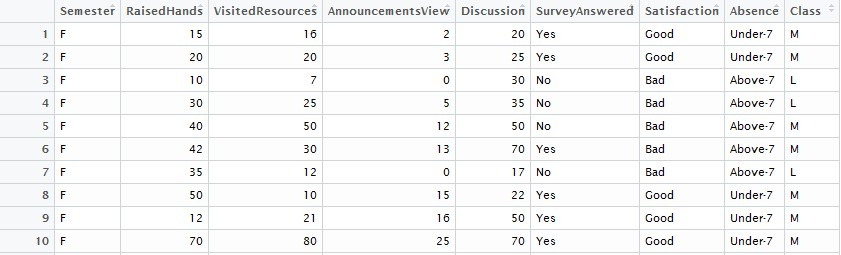
\includegraphics[width=15cm]{tablica.jpg}
\caption{Prvih 10 redaka podatkovnog skupa}
\label{fig:tablica}
\end{figure}
U Tablici~\ref{fig:objašnjenje} ćemo kratko objasniti što koji stupac predstavlja i kojim tipom podatka je opisan:
\begin{table}[H]
\caption{Pročišćavanja podataka}
\begin{tabular}{| l | p{8cm} |}
    \hline
    \textbf{NAZIV ATRIBUTA} & \textbf{OBJAŠNJENJE} \\ \hline
    Semester & Zimski ("F") ili ljetni ("S") semestar \\ \hline
    RaisedHands & Koliko puta je učenik podigao ruku na satu, u vrijednostima 0-100\\ \hline
    VisitedResources & Koliko puta je učenik posjetio dostupne materijale na stranici predmeta, vrijednosti 0-100 \\
    \hline
        AnnouncementsView & Koliko puta je učenik provjerio nove obavijesti na stranici predmeta, vrijednosti 0-100 \\
    \hline
        Discussion & Koliko puta je učenik sudjelovao u diskusijama na predavanjima, vrijednosti 0-100 \\
    \hline
        SurveyAnswered & Jesu li roditelji odgovorili na anketu vezanu za školovanje učenika ("Yes" – Da, "No" – Ne) \\
    \hline
Satisfaction & Jesu li roditelji zadovoljni školom ("Yes" – Da, "No" – Ne) \\
    \hline
        Absence & Koliko puta je učenik izostao s predavanja("Under-7" – Manje od 7 puta, "Above-7" – Više od 7 puta) \\
    \hline
        Class & Broj bodova učenika ("L" – 0-69, "M" – 70-89, "H" – 90-100) \\
    \hline
\end{tabular}
\label{fig:objašnjenje}
\end{table}
U zadnjem koraku u pripremi podataka, provjerit ćemo sadrži li podatkovni skup "NA" vrijednosti naredbom  $any(is.na(data))$. Na izvođenje te naredbe dobili smo odgovor "FALSE", te iz toga zaključujemo da su svi podaci u tablici unutar očekivanih vrijednosti. Time smo odradili i posljednji korak u pripremi, te sada konačno možemo prijeći na analizu podataka.

\section{Predviđanje uspjeha učenika - KNN algoritam}
Prva od metoda koju ćemo koristiti za predviđanje uspjeha učenika je algoritam k-najbližih susjeda(engl. k-nearest neighbors algorithm, KNN). Najjednostavnije objašnjeno, ova metoda primjere iz testnog skupa razmješta na način da uspoređuje atribute s primjerima iz skupa za učenje te one najsličnije grupira zajedno. Iako se jednostavnost ove ideje čini kao vrlo jednostavna, gotovo banalna, algoritam nailazi na široku primjenu, pa tako možemo izdvojiti područja u kojima se koristi:
\begin{itemize}
\item Optičko prepoznavanje znakova i lica u analizi fotografija i videozapisa
\item Predviđanje hoće li se osobi svidjeti neki film prema dosadašnjim dodijeljenim ocjenama (Netflix koristi ovaj algoritam)
\item Pronalaženje obrazaca u genetskom kodu radi prepoznavanja nekih nasljednih bolesti
\end{itemize}
Sada ćemo na primjeru pokazati kako funkcionira KNN algoritam. Iako smo većinu pripreme podataka prethodno obavili, obavit ćemo još par izmjena u podatkovnom skupu kako bismo si olakšali daljnji rad. Učenike, čiji je broj bodova bio okarakteriziran kao "H" odnosno "M" ćemo promatrati na način da su oni prošli predmet, a učenike koji su imali broj bodova "L" ćemo gledati kao da su pali. To ćemo učiniti naredbama na Slici~\ref{fig:nesto}

\begin{figure}[H]
\centering
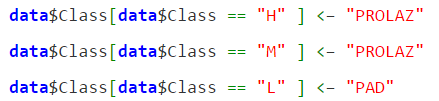
\includegraphics[width=8cm]{nesto1.png}
\caption{Priprema podataka 1}
\label{fig:nesto}
\end{figure}

Također, one učenike koji su izostajali više od 7 dana s predavanja ćemo označiti sa 1, a one koji nisu sa 0, kao što je prikazano na Slici~\ref{fig:nesto2}.
\begin{figure}[H]
\centering
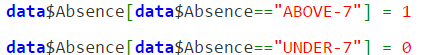
\includegraphics[width=8cm]{nesto2.png}
\caption{Priprema podataka 2}
\label{fig:nesto2}
\end{figure}
Nakon što smo u potpunosti završili s pripremom podataka, sljedeći korak je izgradnja skupa za učenje i testnog skupa. Uobičajeno se kod KNN algoritma taj postupak radi na način da se podatkovni skup podijeli u odnosu 2:1, gdje veći dio pripada skupu za učenje, a manji testnom skupu, pa ćemo tako i mi postupiti.
Naredbama na Slici~\ref{fig:lol} ćemo izgraditi vektor koji sadrži 0.67*480 vrijednosti 1 i 0.33*480 vrijednosti 2 te ga iskoristiti za kreaciju potrebnih skupova. 
\begin{figure}[H]
\centering
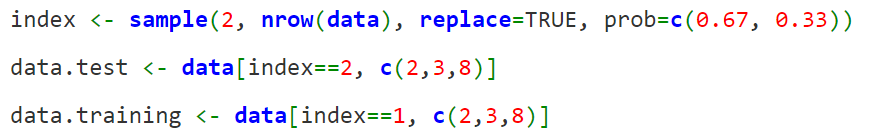
\includegraphics[width=10cm]{lol.png}
\caption{Kreiranje skupa za učenje i trening skupa}
\label{fig:lol}
\end{figure}
Dakle, podskupu data.test smo pridijelili sve vrijednosti kada nam je indeks bio 2, a takvih vrijednosti je bilo 33\% od ukupnog broja(480).  Podskupu data.training, koji predstavlja skup za učenje, smo pridijelili ostalih 67\% vrijednosti. Također, u prethodnim naredbama smo rekli da ćemo pri procjeni učenikova uspjeha koristiti stupce 2, 3 i 8, koji kao što se vidi na Slici~\ref{fig:tablica} redom predstavljaju broj podignutih ruku učenika, broj posjećenih nastavnih materijala i koliko je puta učenik izostao s predavanja. Koristeći upravo te atribute želimo vidjeti koliko dobro je moguće procijeniti uspjeh učenika na kraju godine. Sljedeći korak je izgradnja dva vektora sa vrijednostima učenikova uspjeha ("PROLAZ" ili "PAD"), koje ćemo podijeliti na jednak način kao i prethodne skupove. Broj 9 u naredbama na Slici~\ref{fig:lol2} znači da je stupac koji se procjenjuje na rednom broju 9, a to je upravo učenikov uspjeh.
\begin{figure}[H]
\centering
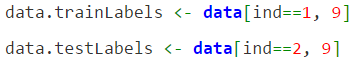
\includegraphics[width=8cm]{lol2.png}
\caption{Vađenje točnih vrijednosti za skup za učenje i trening skup}
\label{fig:lol2}
\end{figure}
Iako smo dosada obavili mnoštvo naredbi, do prave analize odnosno učenja još nije došlo. Zato prelazimo na korak izgradnje klasifikatora(modela), a taj posao nam olakšava ugrađena metoda $knn()$ programskog jezika R. Ta metoda prima 4 argumenta, skup za učenje, testni skup, trening vektor s procjenjivanim vrijednostima i broj k. Brojem k označavamo koliko najbližih susjeda ćemo promatrati. Uobičajeni postupak za odabira broja k vodi se dvjema smjernicama, a to su:
\begin{itemize}
\item uzimanje neparnog broja kako bi se izbjegao "neriješeni" rezultat kod procjene
\item vrijednost broja k bi trebala biti jednaka korijenu duljine skupa za učenje
\end{itemize}
S obzirom da naš skup za učenje sadrži 309 redaka, najbliži neparni korijen tog broja je broj 17, pa ćemo ga iskoristiti kao vrijednost k. Ipak, često se ta praksa zna pokazati i kao pogrešna, pa bismo za svaki slučaj trebali isprobati još nekoliko vrijednosti k, kako bi odabrali najtočniji klasifikator.

\begin{figure}[H]
\centering
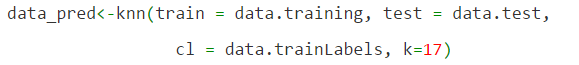
\includegraphics[width=10cm]{lol3.png}
\caption{Izgradnja klasifikatora}
\label{fig:lol3}
\end{figure}
Naredbom na Slici~\ref{fig:lol3} smo izgradili model, te nam je sada ostao zadnji korak, a to je evaluacija, odnosno ocjenjivanje modela. Za to će nam najbolje poslužiti još jedna ugrađena metoda programskog jezika R, a to je $CrossTable($), koja gradi kontingencijsku tablicu. Osnovna verzija ove metode, koja je nama potrebna, prima dva argumenta, a to su: testni vektor s procjenjivanim vrijednostima i izgrađeni model, i izgleda kao na Slici~\ref{fig:lol4}.
\begin{figure}[H]
\centering

\includegraphics[width=10cm]{lol4.png}
\caption{Izrada kontingencijske tablice}
\label{fig:lol4}
\end{figure}
Pozivom ove naredbe dobili smo rezultat prikazan na Slici ~\ref{fig:KNN} i sada ćemo ga objasniti.
\begin{figure}[H]
\centering
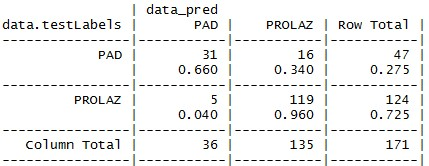
\includegraphics[width=10cm]{KNN.jpg}
\caption{Kontingencijska tablica analize}
\label{fig:KNN}
\end{figure}
Podaci koji se nalaze u prvom redu, označeni kao "TN" i "FP" predstavljaju točne negativne, i lažno pozitivne rezultate. Preciznije to znači da je od 47 učenika koji su pali predmet, naš klasifikator za njih 31 (66\%) to ispravno procijenio, ali je čak kod 16(34\%) učenika napravio pogrešku. Tu količinu pogreške možemo objasniti time da neki od učenika, iako neredovito pohađaju predavanja i vrlo rijetko budu aktivni na satu, samostalno puno vremena posvećuju predmetu te tako uspijevaju osigurati prolaz. Podaci iz drugog reda, označeni s "FN" i "TP" predstavljaju lažno negativne i točno pozitivne rezultate. Kao što vidimo iz tablice, naš klasifikator se puno bolje ponašao u slučajevima kada je trebalo procjenjivati učenike koji su prošli, gdje je pogodio u čak 119 od 124 slučaja (96\%). Možemo zaključiti da klasifikator najbolje funkcionira onda kada stupce s lažno negativnim i lažno pozitivnim rezultatima svedemo na što manji broj. To se može postići isprobavanjem raznih vrijednosti broja k ili standardizacijom po z-vrijednosti, koja izlazi iz domene ovog rada. U Tablici ~\ref{fig:milke} možemo vidjeti da smo došli do sličnih rezultata isprobavanjem drugih vrijednosti broja k, ali nijedan nije uspio nadmašiti prvi dobiveni rezultat gdje smo ,kao što je uobičajeno, za k uzeli korijen duljine skupa za učenje.

\begin{table}[H]
\caption{Pročišćavanja podataka}
\begin{tabular}{| l | l | l | l |}
	\hline
\textbf{K vrijednost} & \textbf{\# lažno negativnih} & \textbf{\# lažno pozitivnih} & \textbf{Postotak netočno procijenjenih} \\ \hline
1            & 15                  & 17                  & 18.71\%                        \\ \hline
5            & 10                  & 22                  & 18.71\%                        \\ \hline
10           & 9                   & 19                  & 16.37\%                        \\ \hline
15           & 8                   & 17                  & 14.62\%                        \\ \hline
17           & 5                   & 16                  & 12.28\%\\ \hline
20           & 8                   & 17                  & 14.62\%\\ \hline
\end{tabular}
\label{fig:milke}
\end{table}

\section{Provjera ovisnosti uspjeha učenika o različitim atributima - Logistička regresija}
U drugom primjeru koristit ćemo metodu logističke regresije. Kod logističke regresije, za razliku od drugih metoda regresije (linearna, polinomna), predviđana varijabla je kategorička i najčešće binarna, što znači da poprima dvije vrijednosti. Logistička regresija koristi se u brojnim područjima, kao što su strojno učenje, razne medicinske discipline i društvene znanosti. Primjerice, u medicini se kod izračuna TRISS-a (Trauma and Injury Severity Score), koji služi za predviđanje smrtnosti ozlijeđenih pacijenata, koristi logistička regresija. Osim toga, logistička regresija često se koristi i kod predviđanja hoće li neka osoba na predsjedničkim izborima glasati za liberalnijeg ili konzervativnijeg kandidata, tako što uzima u obzir brojne karakteristike glasača kao što su: godine, primanja, spol, mjesto stanovanja i slično. U našem slučaju, logističku regresiju koristit ćemo za predviđanje hoće li učenik na kraju semestra proći ili pasti predmet. Za razliku od prvog primjera, ovaj put ćemo sve varijable uzeti kao bitne za određivanje učenikovog uspjeha. Prije samog procesa logističke regresije, kao i u prvom primjeru ćemo atribut učenikova uspjeha preimenovati u "PROLAZ" odnosno "PAD", ali ćemo ovaj put i faktorizirati nenumeričke varijable (SurveyAnswered, Satisfaction, Absence). Nakon što smo to obavili, krećemo s analizom. Za početak ćemo odrediti skup za učenje i testni skup, pri čemu ćemo koristiti sve varijable iz početnog skupa.
Sljedeći korak je izgradnja modela, a on je zajedno s prethodnim korakom prikazan na Slici~\ref{fig:lol5}:
\begin{figure}[H]
\centering
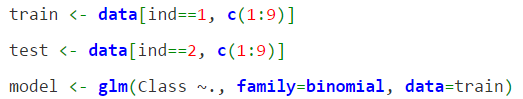
\includegraphics[width=10cm]{lol5.png}
\caption{Izgradnja potrebnih skupova i modela}
\label{fig:lol5}
\end{figure}
U njemu smo prvim parametrom označili da želimo predviđati varijablu Class (uspjeh učenika), drugim da je predviđana varijabla binarnog tipa, a zadnjim smo specificirali skup za učenje. Pozivom naredbe $summary(model)$ dobivamo pojedinosti o modelu na Slici ~\ref{fig:logres1}
\begin{figure}[H]
\centering
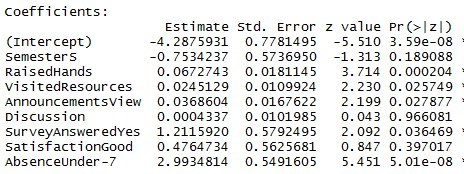
\includegraphics[width=10cm]{logres1.jpg}
\caption{Opis izgrađenog modela}
\label{fig:logres1}
\end{figure}
Kod prikaza pojedinosti modela, najzanimljivi nam je prvi stupac "Estimate".
Što je modul vrijednosti u tom stupcu veći, to znači da ta varijabla ima veći utjecaj na naše predviđanje. Dakle, možemo zaključiti da se uspjeh učenika najbolje može predvidjeti iz toga koliko je izostajao s predavanja i jesu li njegovi roditelji odgovorili na anketu vezanu za školovanje. Daljnji proces logističke regresije ćemo nastaviti koristeći samo te 2 najbitnije varijable, kako bismo izbjegli problem prenaučenosti, koji je ranije objašnjen na primjeru ispod ~\ref{fig:overfit}. Ponovno ćemo izgraditi skup za učenje, testni skup i klasifikator analogno kao i za sve varijable, detaljnije na Slici~\ref{fig:lol6}.
\begin{figure}[H]
\centering
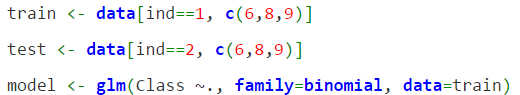
\includegraphics[width=10cm]{lol6.png}
\caption{Izgradnja potrebnih skupova i modela}
\label{fig:lol6}
\end{figure}
Nakon izgradnje modela, moramo ispitati i njegovu preciznost na testnom skupu što ćemo učiniti naredbama navedenim na Slici~\ref{fig:lol7}:
\begin{figure}[H]
\centering
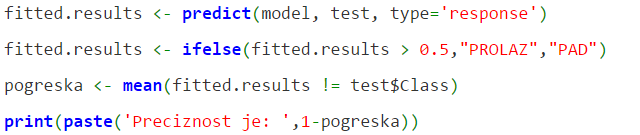
\includegraphics[width=10cm]{lol7.png}
\caption{Procjena ispravnosti odnosno pogreške modela}
\label{fig:lol7}
\end{figure}


Zadnja naredba nam je dala sljedeći ispis:
"Preciznost je:  0.904761904761905"
Što znači da naš klasifikator ispravno predviđa uspješnost studenta na temelju samo dvije varijable u preko 90\% slučajeva. To je zadovoljavajući rezultat i zbog svoje preciznosti, ali i zbog toga što u obzir uzima samo 2 varijable te izbjegava problem prenaučenosti. Preciznost još možemo ispitati i potvrditi i izgradnjom ROC krivulje, koja se tumači na način da veća površina ispod krivulje predstavlja veću preciznost. Krivulja se gradi naredbama prikazanim na Slici~\ref{fig:lol8}
\begin{figure}[H]
\centering
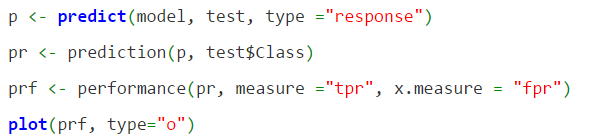
\includegraphics[width=10cm]{lol8.png}
\caption{Prikaz ROC krivulje}
\label{fig:lol8}
\end{figure}

Navedene naredbe crtaju graf na slici ~\ref{fig:logres2} iz kojeg također vidimo da je naš model vrlo ispravan. Točan postotak površine grafa ćemo na način prikazan na Slici\ref{fig:lol9}
\begin{figure}[H]
\centering
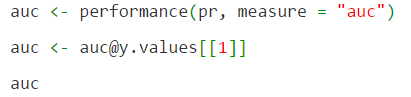
\includegraphics[width=10cm]{lol9.png}
\caption{Računanje površine ROC krivulje}
\label{fig:lol9}
\end{figure}

Navedene naredbe nam daju rezultat 0.938, odnosno još veću preciznost nego smo ju prvotno predvidjeli. 
\begin{figure}[H]
\centering
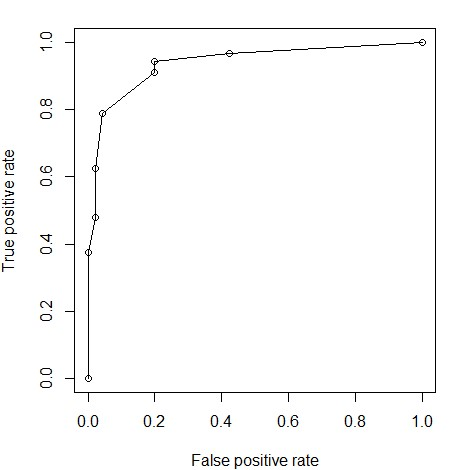
\includegraphics[width=10cm]{logres2.jpg}
\caption{ROC krivulja ispravnosti}
\label{fig:logres2}
\end{figure}

Iz dobivenih rezultata možemo zaključiti da je klasifikacijska analiza može vrlo uspješno primijeniti kod analize podatkovnih skupova iz edukacijske domene, što može biti veoma korisno za poboljšanje kvalitete obrazovnog procesa. Naime, kao što smo vidjeli iz prethodna dva primjera, uspješnost studenta možemo procijeniti s vrlo visokom uspješnošću koristeći samo dva parametra koji ga karakteriziraju. To možemo iskoristiti kako bismo na vrijeme procijenili koji učenici spadaju u "rizičnu" skupinu, odnosno kod kojih učenika je najpotrebnija intervencija i pomoć kako bi se izbjegli negativni rezultati, što u konačnici dovodi do poboljšanja ishoda obrazovnog procesa.
\chapter*{Zaključak}
\addcontentsline{toc}{chapter}{Zaključak}
Kroz ovaj rad smo prošli mnoge teme, počevši od rudarenja podataka pa sve do strojnog učenja, ali smo se na kraju usmjerili na ono što je bio temeljni cilj ovog rada, a to je dubinska analiza podataka iz edukacijske domene (EDM). Zaključili smo da EDM primjenjuje tehnike koje dolaze iz raznih područja (statistika, strojno učenje, dubinska analiza podataka) kako bi procesuirao podatke skupljene tijekom podučavanja, učenja i pisanja raznih oblika provjera. Koristeći te tehnike, obradili smo podatkovni skup te došli do rezultata koji su u potpunosti ispunili naš prvotni cilj, a to je bio predviđanje uspjeha učenika s vrlo visokom preciznošću koristeći se parametrima koji ih karakteriziraju. Korištenjem metode linearne regresije i algoritma k-najmanjih kvadrata (KNN), uspješnost studenta (prolaz/pad) smo procjenjivali s preciznošću od 93\%(logistička regresija) odnosno 89\%(KNN). Ipak, bez obzira na vrlo uspješne rezultate,  polje EDM-a je još uvijek prilično mlada znanstvena disciplina i još je puno vremena i posla potrebno obaviti kako bi se ono počelo shvaćati kao zrela disciplina. Za to je potrebno osim brojnih znanstvenika, u proces analize uključiti i profesore te obrazovne institucije. Također, nužno je pokušati prebaciti EDM iz laboratorijskih uvjeta na otvoreno tržište, jer je to jedan od najčešćih uvjeta uspjeha u današnje vrijeme. Da bi se to postiglo, potrebno je brojne alate potrebne za EDM učiniti besplatnim ili ih ponuditi kao softver s otvorenim kodom (engl. open source software) te nakon toga kroz razne tipove tečajeva upoznati moguće korisnike i olakšati im rad sa spomenutim alatima.

\bibliography{literatura}
\bibliographystyle{fer}

\begin{sazetak}
U ovom radu obradili smo proces dubinske analize podataka u edukacijskoj domeni (EDM). Kroz prvih par poglavlja, fokusirali smo se na znanstvene discipline iz kojih je proizašao i čijim se metodama koristi EDM, a to su rudarenje podataka i strojno učenje. Također, objasnili smo i kako se razvijalo polje EDM-a te pristupe koji se koriste u analizi. U zadnjem poglavlju smo odradili praktični dio završnog rada, a to je primjena klasifikacijskih metoda kod dubinske analize podataka u edukacijskoj domeni. Analize smo proveli koristeći programski jezik R i dva klasifikacijska algoritma (k-NN algoritam i logistička regresija) te smo prikazali njihov način učenja, a u konačnici i rezultate (uspješnost učenja) tih algoritama.

\kljucnerijeci{dubinska analiza podataka u edukacijskoj domeni, otkrivanje znanja u skupovima podataka, strojno učenje, klasifikacijska analiza, programski jezik R}
\end{sazetak}


\bigbreak
\engtitle{Application of Classification Analysis in the Educational Domain}
\begin{abstract}
In this thesis we have described the educational data mining process. Through the first few chapters, our main focus was on science fields which have preceded and whose methods are used in EDM, which are data mining and machine learning. Also, we have explained development of EDM and main approaches that are used in analysis. In the last chapter we did the practical part of this work, and that was application of classification methods in educational data mining. Analysis were conducted using programming language R and two classification algorithms (k-NN algorithm and logistic regression) and in those analysis we have shown in which way are these algorithms learning and results (level of success) which they produce.

\keywords{educational data mining, knowledge discovery in databases, machine learning, classification analysis, programming language R}
\end{abstract}

\end{document}
